\documentclass[utf8]{beamer}

%%%% PACKAGES, ENVIRONMENTS & COMMANDS
\usepackage{textpos}
\usepackage{textcomp}
\usepackage{tikz}

\newcommand\RBox[1]{%
  \tikz\node[draw,rounded corners,align=center,] {#1};%
}
\newcommand{\okeanos}{\url{~}okeanos}

%%%% THEMES
\mode<presentation>
{
  \usetheme{CambridgeUS}
  \usecolortheme{dolphin}

  \setbeamercovered{transparent}
  % or whatever (possibly just delete it)
}

\usebackgroundtemplate%
{%
    
\includegraphics[width=\paperwidth,height=\paperheight]{template/grnet_background.pdf}%
}

\setbeamerfont{institute}{size=\large}

\title[Archipelago]{Archipelago:\\ New Cloud Storage Backend of GRNET}

\author[F. Giannakos \and C. Nanakos]
{%
  \texorpdfstring{
    \begin{columns}
      \column{.45\linewidth}
      \centering
      \RBox{Filippos  Giannakos\\
      \href{mailto:philipgian@grnet.gr}{philipgian@grnet.gr}}
      \column{.45\linewidth}
      \centering
      Chrysostomos Nanakos\\
      \href{mailto:cnanakos@grnet.gr}{cnanakos@grnet.gr}
    \end{columns}
  }
  {foo}
}

\date[$16^{th}$ TF-Storage, Feb.\ 13, 2015]{$16^{th}$ TF-Storage Meeting \\
February 13, 2015}
\institute[GRNET]{Greek Research and Technology Network (GRNET) S.A.}

\subject{Talks}
% This is only inserted into the PDF information catalog. Can be left
% out.

% If you have a file called "university-logo-filename.xxx", where xxx
% is a graphic format that can be processed by latex or pdflatex,
% resp., then you can add a logo as follows:

% \pgfdeclareimage[height=0.5cm]{university-logo}{university-logo-filename}
% \logo{\pgfuseimage{university-logo}}

\titlegraphic{
  \colorbox{white}{
\includegraphics[width=3cm]{template/grnet-logo-en.pdf}}
}

% If you wish to uncover everything in a step-wise fashion, uncomment
% the following command:

%\beamerdefaultoverlayspecification{<+->}

%%%% SLIDES
\begin{document}

%%---------- Title-page ----------
\begin{frame}
  \begin{textblock*}{3cm}(.75\textwidth,8cm)
    
\includegraphics[width=3cm]{template/logos-all.jpg}
  \end{textblock*}

  \titlepage
\end{frame}

%%---------- Slides ----------

%% Background & Motivation
%%%%%%%%%%%%%%%%%%%%%%%%%%%%%%%%%%%%%%%%%%%%%%%%%%%%%%%%%%%%%%%%%%%%%%%%%%%%%%%%
\section{Background \& Motivation}

\subsection{Background}

\begin{frame}{Background}
  \begin{textblock*}{3cm}(.70\textwidth,.75cm)
    
\includegraphics[width=3cm]{figures/synnefo-logo.pdf}
  \end{textblock*}

  \begin{textblock*}{3cm}(.70\textwidth,1.75cm)
    
\includegraphics[width=3cm]{figures/okeanos-logo.pdf}
  \end{textblock*}

  \begin{textblock*}{3cm}(.70\textwidth,2.75cm)
    
\includegraphics[width=3cm]{figures/okeanos-global.png}
  \end{textblock*}

  \begin{itemize}
  \item Synnefo
    \begin{itemize}
      \item OpenStack compatible cloud platform
    \end{itemize}
  \item Powers:
    \begin{itemize}
    \item \okeanos\\
      \url{https://okeanos.grnet.gr}
    \item \okeanos-global\\
      \url{https://okeanos-global.grnet.gr}
    \end{itemize}
  \end{itemize}
\end{frame}

\subsection{Motivation}

\begin{frame}{Motivation}
  \begin{itemize}
  \item Pithos
    \begin{itemize}
      \item Uploaded Files / Images
    \end{itemize}
  \item Plankgton
    \begin{itemize}
      \item Registered Images
    \end{itemize}
  \item Cyclades
    \begin{itemize}
      \item Virtual Disks
    \end{itemize}
  \end{itemize}
\end{frame}

\begin{frame}{Unified View of Storage Resources}
\begin{columns}
  \column{.10\linewidth}
  
\includegraphics[width=1cm]{figures/files.png}\\[1em]

  
\includegraphics[width=1cm]{figures/images.png}\\[1em]

  
\includegraphics[width=1cm]{figures/volumes.png}\\[1em]

  
\includegraphics[width=1cm]{figures/snapshots.png}
  \column{.75\linewidth}
  \begin{itemize}
  \item Files\\
    User files, with Dropbox-like syncing.\\[1em]
  \item Images\\
    Templates for VM creation.\\[1em]
  \item Volumes\\
    Live disks, as seen from VMs.\\[1em]
  \item Snapshots\\
    Point in time snapshots of volumes.
  \end{itemize}
\end{columns}
\end{frame}

%% Archipelago Features
%%%%%%%%%%%%%%%%%%%%%%%%%%%%%%%%%%%%%%%%%%%%%%%%%%%%%%%%%%%%%%%%%%%%%%%%%%%%%%%%
\section{Archipelago Features}

\subsection{Storage Features}

\begin{frame}{Archipelago}
  \begin{itemize}
    \item Storage Virtualization System
      \begin{itemize}
        \item Powering storage in Synnefo
      \end{itemize}
    \item Decouples storage resources from storage backends
      \begin{itemize}
        \item Files / Images / Volumes / Snapshots
      \end{itemize}
    \item Unified way to provision, handle, and present resources
    \item Decouples logic from actual physical storage
      \begin{itemize}
        \item Software-Defined Storage
      \end{itemize}
  \end{itemize}
\end{frame}

\begin{frame}{Backend Agnostic}
  \begin{itemize}
    \item Advantages:
      \begin{itemize}
      \item No vendor lock-in
      \item Migration from one storage backend to another
      \item Possibility of combining backends
    \end{itemize}
    \item \okeanos{} started with NFS and migrated to RADOS
  \end{itemize}
\end{frame}

\begin{frame}{Storage Backend for the Cloud}
  \begin{itemize}
  \item With Archipelago we offer:
    \begin{itemize}
      \item Deduplication
      \item Syncable File/Image upload with partial upload
      \item Image Registration
      \item Thin clones
      \item Downloadable thin snapshots
    \end{itemize}
  \item with zero data movement.
  \end{itemize}
\end{frame}

\subsection{Services Overview}

\begin{frame}{Services Overview}
  \begin{center}
    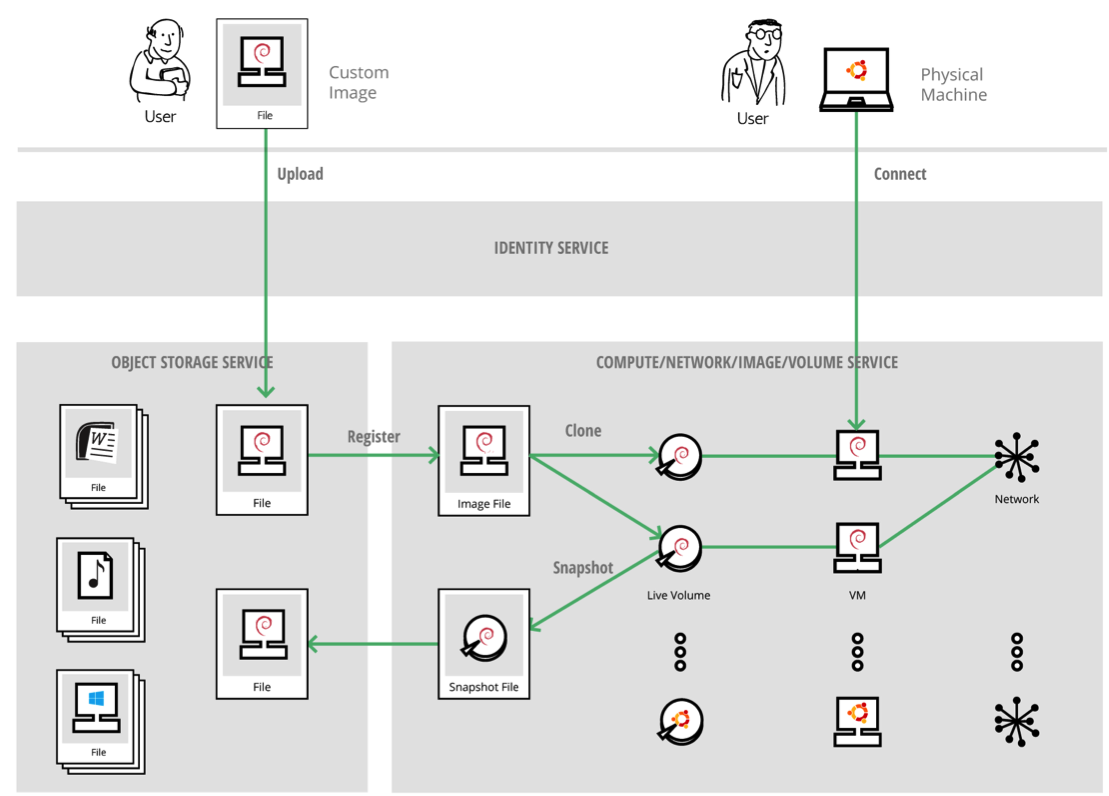
\includegraphics[width=.85\linewidth]{figures/services.png}
  \end{center}
\end{frame}

%% Under the Hood
%%%%%%%%%%%%%%%%%%%%%%%%%%%%%%%%%%%%%%%%%%%%%%%%%%%%%%%%%%%%%%%%%%%%%%%%%%%%%%%%
\section{Under the Hood}

\subsection{Everything is a Resource}

\begin{frame}{How it is Done}
  \begin{itemize}
    \item Everything is a resource on Archipelago
    \item The \alert{same} resource is exposed as:
      \begin{itemize}
        \item A file through the API of the Storage Service (Pithos)
        \item An image through the API of the Image Service
        \item A live disk / VM volume through the API of the Volume Service
        \item A snapshot through the API of the Volume Service
      \end{itemize}
      \item All data remain in one place
      \item No copying of data around
    \end{itemize}
\end{frame}

\subsection{Mapfiles}

\begin{frame}{Mapfiles}
  \begin{itemize}
  \item Mapfile for each resource
    \begin{itemize}
      \item Keeps track of the mappings from resource offset to objects
      \item Keeps metadata information for each resource
    \end{itemize}
  \item Operates on mapfiles
  \end{itemize}
\end{frame}

\begin{frame}{From Mapfiles to Data}
  \begin{center}
    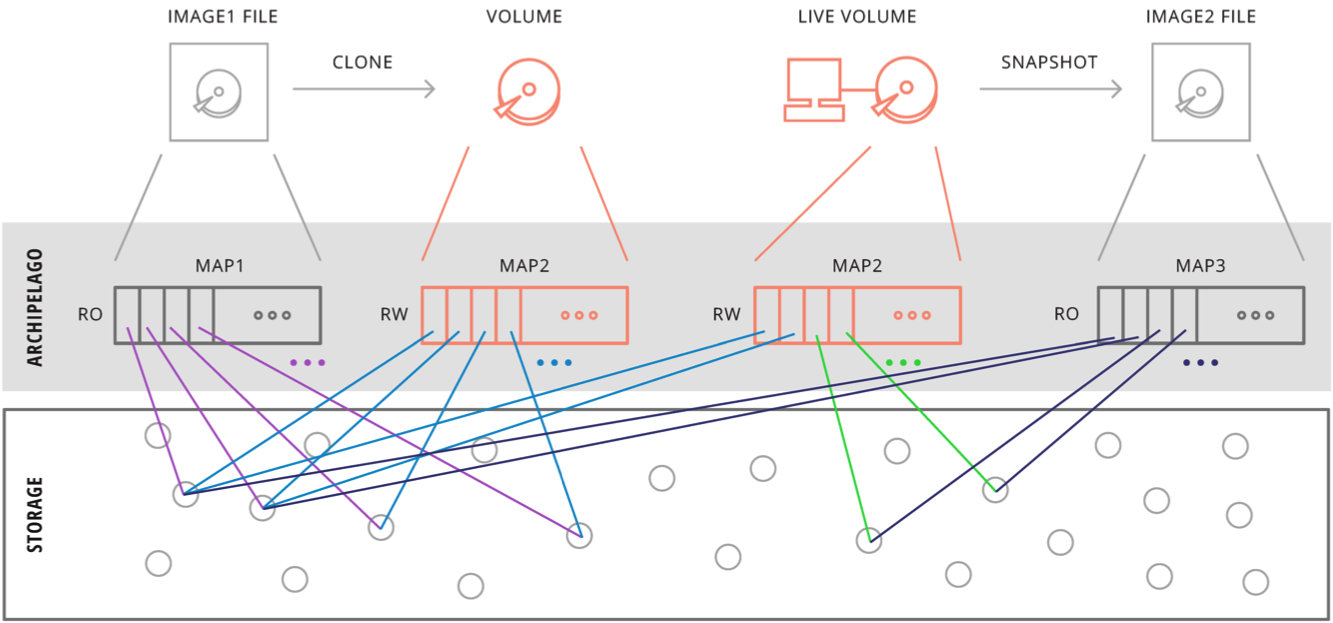
\includegraphics[width=.90\linewidth]{figures/mapfiles.png}
  \end{center}
\end{frame}

\subsection{Architecture}

\begin{frame}{High Level Architecture}
  \begin{center}
    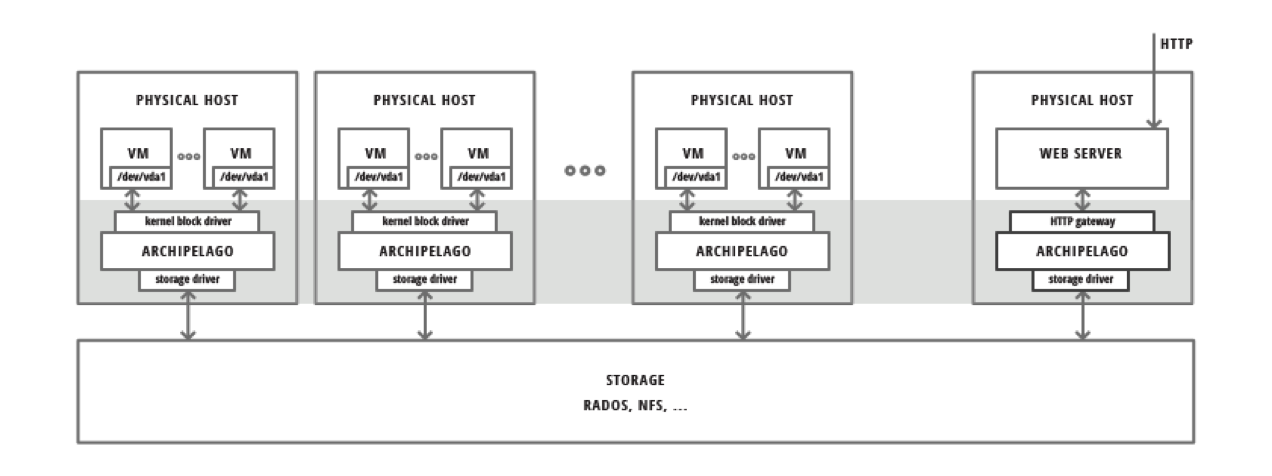
\includegraphics[width=.90\linewidth]{figures/high-architecture.png}
  \end{center}
\end{frame}

\begin{frame}{Low level Architecture}
  \begin{center}
    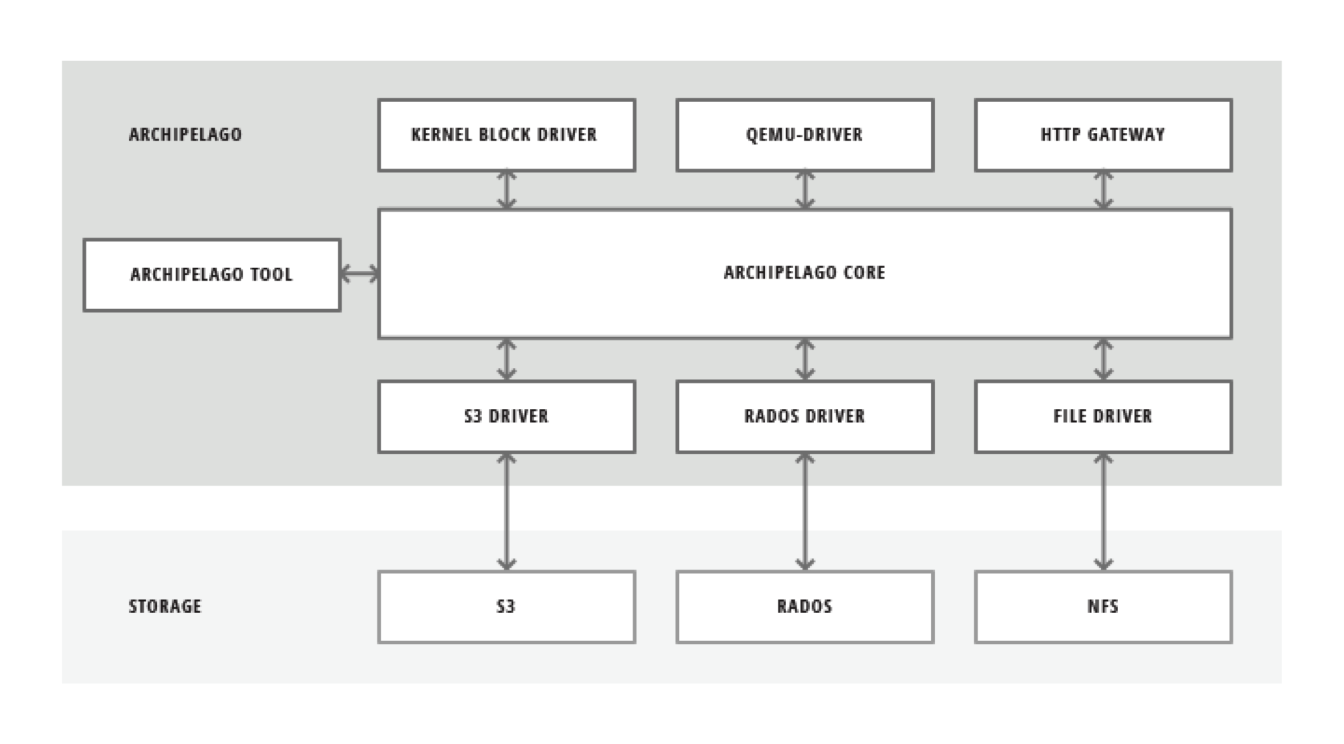
\includegraphics[width=.90\linewidth]{figures/low-architecture.png}
  \end{center}
\end{frame}

\begin{frame}{Core}
  \begin{itemize}
    \item Volume composer
      \begin{itemize}
      \item Composes resource I/O from individual objects
      \end{itemize}
    \item Mappe
      \begin{itemize}
      \item Keeps and updates the mappings from volume offsets to
        individual objects which actually hold the data
      \end{itemize}
    \item Flexible I/O pipeline
      \begin{itemize}
      \item Can be extended with other components offering common
        functionality
      \end{itemize}
  \end{itemize}
\end{frame}

\subsection{Interfaces}

\begin{frame}{Client Endpoints}
  \begin{itemize}
  \item Upstream Native QEMU virtio driver
    \begin{itemize}
    \item VM interface
    \end{itemize}
  \item Blktap2 driver
    \begin{itemize}
    \item Admin/VM interface
    \end{itemize}
  \item Pithos
    \begin{itemize}
    \item Web interface
    \end{itemize}
  \end{itemize}
\end{frame}

\begin{frame}{Backend Drivers}
  \begin{itemize}
    \item Currently supported backends:
      \begin{itemize}
      \item Files (Any FS with POSIX semantics)
      \item RADOS (Using native librados interface)
      \item GlusterFS (Using native libgfapi interface)
      \end{itemize}
    \item Future: Anything that can support object semantics
  \end{itemize}
\end{frame}

%% Advantages over other Solutions
%%%%%%%%%%%%%%%%%%%%%%%%%%%%%%%%%%%%%%%%%%%%%%%%%%%%%%%%%%%%%%%%%%%%%%%%%%%%%%%%
\section{Advantages over other Solutions}

\begin{frame}{Advantages over other Solutions}
\begin{itemize}
  \item Allows for resource compositions from already existing objects
  \item Unified view of all cloud resources
\end{itemize}
\end{frame}

%% Experience
%%%%%%%%%%%%%%%%%%%%%%%%%%%%%%%%%%%%%%%%%%%%%%%%%%%%%%%%%%%%%%%%%%%%%%%%%%%%%%%%
\section{Experience}

\begin{frame}{Experience from Production}
\begin{itemize}
  \item 3000 VM volumes
  \item $\approx$2.8M user uploaded files
  \item $\approx$25TB deduplicated data
  \item 22M actual objects on the storage backend
\end{itemize}
\end{frame}

%% The Future
%%%%%%%%%%%%%%%%%%%%%%%%%%%%%%%%%%%%%%%%%%%%%%%%%%%%%%%%%%%%%%%%%%%%%%%%%%%%%%%%
\section{The Future}

\begin{frame}{Upcoming Features}
  \begin{itemize}
    \item New mapfile format
      \begin{itemize}
      \item More compact
      \item Allows for larger volumes with minimal metadata overhead
      \end{itemize}
    \item Garbage collection
      \begin{itemize}
      \item Deferred reference counting
      \item Automatic deletion of unused objects
      \end{itemize}
    \end{itemize}
\end{frame}

%% Thanks
%%%%%%%%%%%%%%%%%%%%%%%%%%%%%%%%%%%%%%%%%%%%%%%%%%%%%%%%%%%%%%%%%%%%%%%%%%%%%%%%
\section{Thanks}

\begin{frame}{Thanks}

\end{frame}


\end{document}
